\documentclass[12pt]{article}

\usepackage[a4paper]{geometry}
\usepackage[utf8]{inputenc}
\usepackage[english]{babel}
\usepackage[automark]{scrpage2}
\usepackage{listings}
\usepackage{hyperref}
\usepackage{xcolor}
\usepackage{caption}
\usepackage{graphicx}

\pagestyle{scrheadings}
\clearscrheadfoot
\ihead[]{RoboSoccer Laboratory}
\ohead[]{Team C}
\cfoot[]{\pagemark}


\begin{document}

\section{Project plan}
\subsection{Definition of the project objectives}
The main project objective is winning the "RoboSoccer Championship" at the end of this course. 
This requires the implementation of low- and mid-level robot controls and an artificial intelligence with good tactics.

In addition the programm has to obey the RoboSoccer rules during the match and has to have a penalty-shoot-out mode.

\subsection{Framework and Procedure}
\subsubsection*{Hardware}
One team controlls three modded Pololu 3pi robots to shoot a golfball into the goal of the enemy.
They are connected to a server via bluetooth and located using a firewire camera above of the playground.

\subsubsection*{Team Members}
\begin{itemize}
	\item Markus Hofbauer
	\item He Jiang
	\item Kevin Meyer
	\item Benedikt Schmidt
	\item Florian Wirnshofer
\end{itemize}

\subsubsection*{Team Organisation}
\begin{itemize}
	\item \textbf{Internal Communication}
	\begin{itemize}
		\item Team Discussion Board \\\mbox{(phpBB: \textit{https://forum.kevin-meyer.de})}
		\item Email
	\end{itemize}
	\item \textbf{Weekly Jour Fixe} at Laboratory or Eikon
	\item Additional meetings on demand
\end{itemize}

\subsubsection*{Software}
\begin{itemize}
	\item \textbf{Target and Development-OS:} Linux
	\item \textbf{IDE:} Qt Creator
	\item \textbf{VCS:} Git (hosted on \textbf{bitbucket.org})
	\item \textbf{Build System:} CMake
\end{itemize}

\subsection{Tasks}
\textit{Maybe add something about the "Spiral-Modell"}
The project is based on the spiral model with the following milestones:
\begin{itemize}
	\item \textbf{Deadline: \textcolor{red}{07.05.2014}}
	\begin{itemize}
		\item Kickoff Position
		\item Goalkeeper
		\item Penalty Shooting
	\end{itemize}
	
	\item \textbf{Deadline: \textcolor{red}{04.06.2014}}
	\begin{itemize}
		\item Collision Avoidance
		\item Ball Control
		\item Player Interaction
	\end{itemize}
	
	\item \textbf{Strategy and Tactics}\\
	\textbf{Deadline: \textcolor{red}{25.06.2014}}
	
	\item \textbf{RoboSoccer Championship}\\
	\textbf{Deadline: \textcolor{red}{02.07.2014}}
\end{itemize}

\subsection{Resource plan}

\begin{itemize}
	\item \textbf{PM:}  
	\item \textbf{QM:} 
	\item \textbf{CM:} 
	\item \textbf{SE:} 
	\item \textbf{SA:} 
\end{itemize}
\textit{Add unique and team responsibilities and tasks.}

\subsection{Time scedule}
\textit{Insert Gantt Chart here.}\\
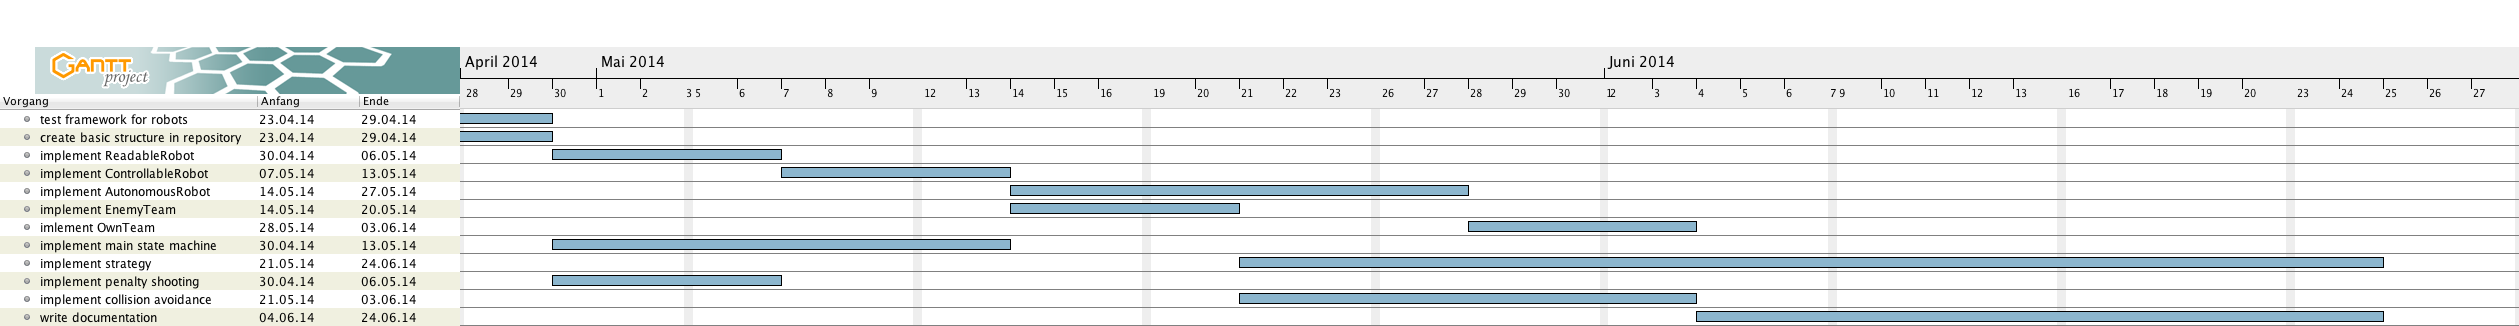
\includegraphics[width=\textwidth]{../ganttchart.png}

\subsection{Cost plan}
\textit{Your advertisement could be here.}

\subsection{Implementation Draft}
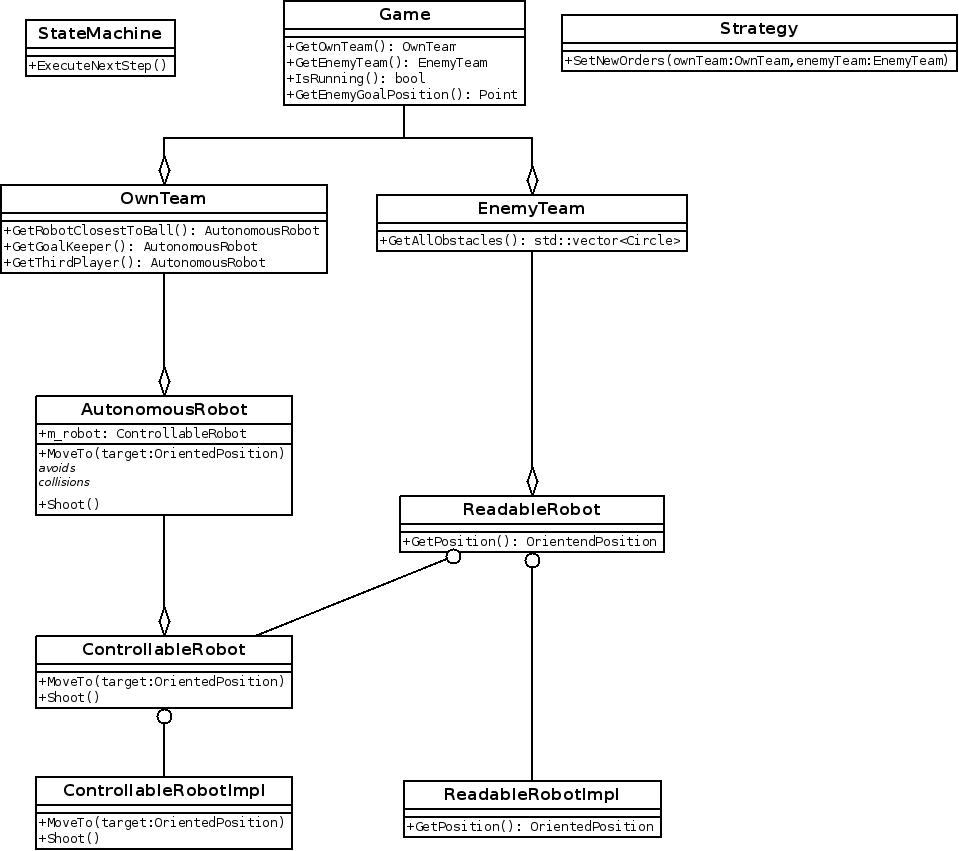
\includegraphics[width=\textwidth]{../architecture.jpeg}

\end{document}
